\header{
    \section{La chartreuse} \label{la-chartreuse}
    %
    
    \insertComment{Sur l'air de "Banana Split" de Lio (1980).}{}
}

\enluminure{4}{\href{https://www.youtube.com/watch?v=bsqLi9LfiwM}{Q}}{uand} chui arrivée ici
\\J'étais un peu aigrie
\\Je n'étais pas heureuse,
\\Ch'connaissais pas la chartreuse
\\J'ai pas testé tout de suite, 
\\J'avais peur de m'prendre une cuite
\\Oui une cuite, oui une cuite, oui une cuite, une cuite, une cuite...
\\\\\textbf{Refrain :}
\bisdouble{C'est la boisson aux plantes des faluchards Grenoblois}
{Baptême, Sono ou bien congrès de toute façon t'y a droit}
\\La la chartreuse, la la chartreuse, ca rend heureuse Hou !~~ \bissimple
\\\\Il y'en a plusieurs sortes, 
\\Celle que j'préfère c'est la jaune,
\\Elle pique un peu la gorge, 
\\Et puis après elle rend stone
\\Mais j'bois pas jusqu'à l'ivresse, 
\\Si non c'est la PLS
\\PLS PLS PLS LS LS LS LS ...
\\\\Une fois qu't'y a gouté, 
\\Ben tu peux plus t'en passer
\\Si tu n'as pas ta dose, 
\\Tu d'viens complèt'ment morose
\\C'est bien pour s'amuser, 
\\Mais faut pas en abuser
\\Abuser, abuser, abuser, buser, buser, buser...
\breakpage
Et si tu fais d'la merde, 
\\C'est pas d'sa faute à elle
\\Apprends a te gérer, 
\\Putain montre pas tes nénés
\\Ton cul ou bien ta bite, 
\\Dépêche toi range moi ca vite
\\Vite vite vite vite vite vite vite vite vite vite...
\\\\Au fait les Parisiens, 
\\Vous savez on vous aime bien
\\Mais cette recette de fou, 
\\Et ben elle est à nous
\\Et pas d'négociations, 
\\Vous savez qu'on a raison
\\N'a raison, n'a raison, n'a raison, raison, raison, raison...
\begin{center}
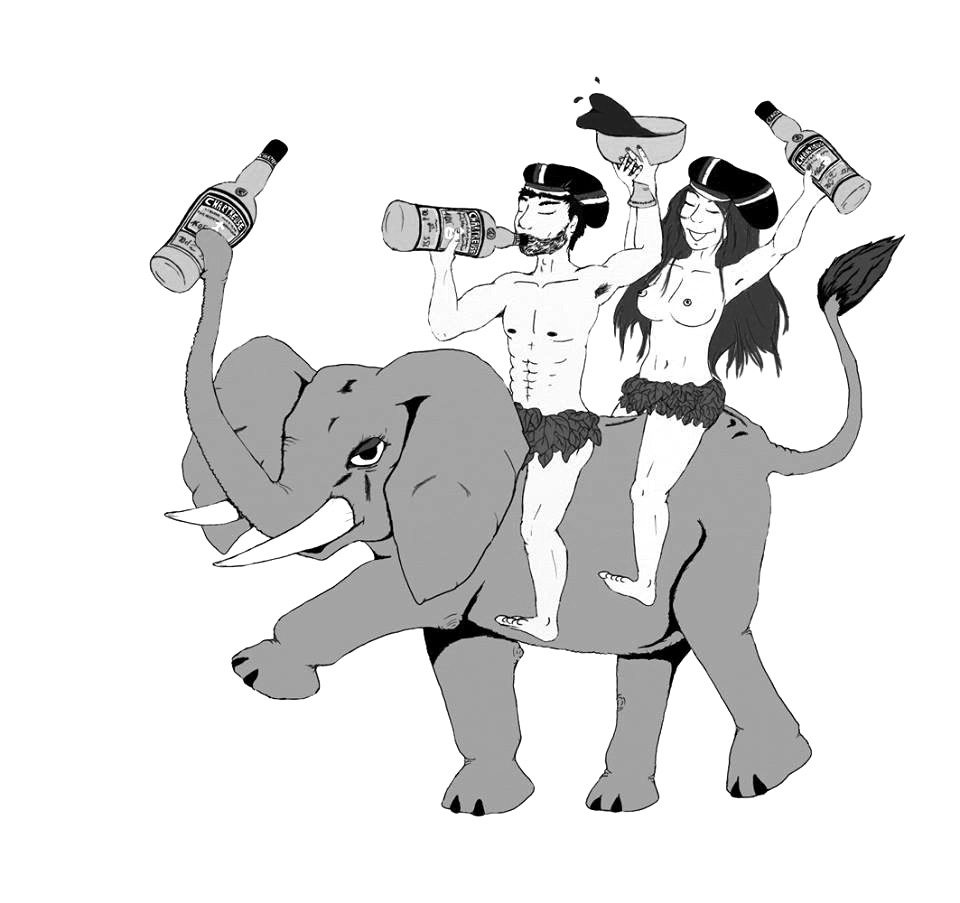
\includegraphics[width=1\textwidth]{images/chartreuse2.jpg}
\end{center}

\breakpage